\documentclass[10pt,a4paper,spanish]{report}

\usepackage[spanish]{babel}
\usepackage[utf8]{inputenc}
\usepackage{amsmath, amsthm}
\usepackage{amsfonts, amssymb, latexsym}
\usepackage{enumerate}
\usepackage[official]{eurosym}
\usepackage{graphicx}
\usepackage[usenames, dvipsnames]{color}
\usepackage{colortbl}
\usepackage{multirow}
\usepackage{fancyhdr}
\usepackage[all]{xy}
\usepackage{pgfplots}
\usepackage{algpseudocode}
\usepackage{listings}
\usepackage{titlesec}
\usepackage{minted}
\usepackage{adjustbox}

\pgfplotsset{compat=1.5}

% a4large.sty -- fill an A4 (210mm x 297mm) page
% Note: 1 inch = 25.4 mm = 72.27 pt
%       1 pt = 3.5 mm (approx)

% vertical page layout -- one inch margin top and bottom
\topmargin      0 mm    % top margin less 1 inch
\headheight     0 mm    % height of box containing the head
\headsep       10 mm    % space between the head and the body of the page
\textheight   250 mm
\footskip      14 mm    % distance from bottom of body to bottom of foot

% horizontal page layout -- one inch margin each side
%\oddsidemargin    0   mm    % inner margin less one inch on odd pages
%\evensidemargin   0   mm    % inner margin less one inch on even pages
%\textwidth      159.2 mm    % normal width of text on page

\usepackage[math]{iwona}
\usepackage[T1]{fontenc}
\usepackage{inconsolata}

\usepackage[pdftex, bookmarks=true,
	bookmarksnumbered=false, % true means bookmarks in
	% left window are numbered
	bookmarksopen=false,     % true means only level 1
	% are displayed.
	colorlinks=true,
linkcolor=webblue]{hyperref}

\definecolor{webgreen}{rgb}{0, 0.5, 0} % less intense green
\definecolor{webblue}{rgb}{0, 0, 0.5}  % less intense blue
\definecolor{webred}{rgb}{0.5, 0, 0}   % less intense red
\definecolor{dblackcolor}{rgb}{0.0,0.0,0.0}
\definecolor{dbluecolor}{rgb}{.01,.02,0.7}
\definecolor{dredcolor}{rgb}{0.8,0,0}
\definecolor{dgraycolor}{rgb}{0.30,0.3,0.30}

\newcommand{\HRule}{\rule{\linewidth}{0.5mm}} % regla horizontal para  el titulo

\pagestyle{fancy}
%con esto nos aseguramos de que las cabeceras de capítulo y de sección vayan en minúsculas

\renewcommand{\chaptermark}[1]{%
	\markboth{#1}{}}
\renewcommand{\sectionmark}[1]{%
	\markright{\thesection\ #1}}
\fancyhf{} %borra cabecera y pie actuales
\fancyhead[LREO]{\bfseries\thepage}
\fancyhead[LO]{\bfseries\leftmark}
\renewcommand{\headrulewidth}{0.5pt}
\renewcommand{\footrulewidth}{0pt}
\addtolength{\headheight}{0.5pt} %espacio para la raya
\fancypagestyle{plain}{%
	\fancyhead{} %elimina cabeceras en páginas "plain"
	\renewcommand{\headrulewidth}{0pt} %así como la raya
}

%%%%% Para cambiar el tipo de letra en el título de la sección %%%%%%%%%%%
\usepackage{sectsty}
\chapterfont{\fontfamily{pag}\selectfont} %% for chapter if you want
\sectionfont{\fontfamily{pag}\selectfont}
\subsectionfont{\fontfamily{pag}\selectfont}
\subsubsectionfont{\fontfamily{pag}\selectfont}
\titleformat{\chapter}{\normalfont\Huge}{}{0pt}{\Huge} % Capítulos sin "Capítulo x" encima del título

\renewcommand{\labelenumi}{\arabic{enumi}. }
\renewcommand{\labelenumii}{\labelenumi\alph{enumii}) }
\renewcommand{\labelenumiii}{\labelenumii\roman{enumiii}: }

\newmintedfile[mypython]{python}{
	frame=lines,
	framesep=2mm,
	baselinestretch=1.2,
	bgcolor=LightGray,
	fontsize=\footnotesize,
	linenos
}

\title{Seguridad y Protección de Sistemas Informáticos \\
Certificados Digitales}
\author{David Sánchez Jiménez}

\begin{document}
\begin{titlepage}
 \begin{center}
  \HRule \\[0.8cm]
  \textsc{\huge Seguridad y Protección \\ de Sistemas Informáticos \\[0.5cm] Puzles Hash}\\[1.6cm]
  \HRule \\[1cm]
  \begin{flushleft}
   \emph{Hecho por:}\\
   David Sánchez Jiménez
  \end{flushleft}
  \vspace{12cm}
  \large{\today}\\
  \vspace{0.5cm}
  \htmladdnormallink{
\includegraphics[width=2cm]{Imagenes/88x31.png}}
  {http://creativecommons.org/licenses/by-nc/4.0/}\\[0.5cm]
  \texttt{Prácticas de Seguridad y Protección de Sistemas Informáticos\\ by
   \href{mailto:dasaji92@gmail.com}{David Sánchez Jiménez} is licensed under a \htmladdnormallink{Creative Commons Reconocimiento-NoComercial-CompartirIgual 4.0 Internacional License}
   {http://creativecommons.org/licenses/by-nc/4.0/}}.\\[3mm]
 \end{center}
\end{titlepage}

\tableofcontents
\newpage

% ----------------------------------------------------------------
\chapter{Ejercicio 1}

\section{Enunciado}
\noindent
Elegid una función hash H con salida de n-bits con n $\leq$ 256. Para la función H, realizad, en el lenguaje de programación que queráis, una función que tome como entrada un texto y un número de bits b. Creará un id que concatene una cadena aleatoria de n bits con el texto. Pegará a ese id cadenas aleatorias x de n bits hasta lograr que H(id||x) tenga sus primeros b bits a cero. La salida será el id, la cadena x que haya proporcionado el hash requerido, el valor del hash y el número de intentos llevados a cabo hasta encontrar el valor x apropiado.

\section{Respuesta}
\noindent

\begin{minted}[linenos,numbersep=5pt,gobble=0,frame=lines,framesep=2mm,]{python}
	import formatter
	import hashlib
	import random
	import sys
	from itertools import groupby


	def rand_bits_number():
	    return str(random.getrandbits(256))


	def concatenate(text, number_string):
	    return number_string + text


	def hash_puzzle(concatenation):
	    return hashlib.sha256(concatenation.encode('utf-8 ')).hexdigest()


	def hex_to_bin(hexadecimal):
	    return bin(int('1' + hexadecimal, 16))[3:]


	def print_results(identification, x, h, b, steps):
	    print("\nID: ", identification, "\nX: ",
	          x, "\nHash: ", h, "\nBinary: ", b, "\nSteps: ", steps)


	def puzzle(text, num_bits):
	    condition = False
	    steps = 0
	    number_string = rand_bits_number()
	    identification = concatenate(text, number_string)

	    while condition != True:
	        x = rand_bits_number()
	        concatenation = concatenate(text, x)
	        h = hash_puzzle(concatenation)
	        b = hex_to_bin(h)

	        if len(b.split("1", 1)[0]) == num_bits:
	            steps += 1
	            condition = True
	        else:
	            steps += 1

	    print_results(identification, x, h, b, steps)


	if __name__ == '__main__':
	    text = open(sys.argv[1], mode='r', encoding='UTF-8')
	    num_bits = sys.argv[2]
	    puzzle(text.read(), int(num_bits))

\end{minted}

% ----------------------------------------------------------------
\chapter{Ejercicio 2}

\section{Enunciado}
\noindent
Calculad una tabla/gráfica que vaya calculando el número de intentos para cada valor de b. Con el objeto de que los resultados eviten ciertos sesgos, para cada tamaño b realizad el experimento 10 veces y calculad la media del número de intentos.

\section{Respuesta}
\noindent
Los valores obtenidos tras ejecutar el programa son los siguientes:

\begin{table}[h!]
 \centering
 \begin{adjustbox}{max width=\textwidth}
  \begin{tabular}{*{14}{|c}|} %{|c|c|c|c|c|c|c|c|c|c|c|c|}
   \hline
   \textbf{Nº de Ceros / Intentos} & \textbf{1} & \textbf{2} & \textbf{3} & \textbf{4} & \textbf{5} & \textbf{6} & \textbf{7} & \textbf{8} & \textbf{9} & \textbf{10} & \textbf{Media}      \\ \hline
   \textbf{1}                      & 12         & 1          & 4          & 11         & 1          & 4          & 5          & 1          & 11         & 3           & \textbf{5,3}        \\ \hline
   \textbf{2}                      & 7          & 7          & 1          & 4          & 9          & 2          & 4          & 19         & 1          & 6           & \textbf{6}          \\ \hline
   \textbf{3}                      & 118        & 15         & 13         & 4          & 10         & 24         & 8          & 24         & 68         & 2           & \textbf{28,6}       \\ \hline
   \textbf{4}                      & 10         & 19         & 118        & 37         & 15         & 3          & 44         & 8          & 15         & 36          & \textbf{30,5}       \\ \hline
   \textbf{5}                      & 20         & 23         & 119        & 50         & 4          & 75         & 36         & 18         & 159        & 170         & \textbf{67,4}       \\ \hline
   \textbf{6}                      & 42         & 26         & 277        & 84         & 40         & 175        & 61         & 85         & 86         & 93          & \textbf{96,9}       \\ \hline
   \textbf{7}                      & 150        & 207        & 717        & 591        & 832        & 320        & 14         & 218        & 321        & 332         & \textbf{370,2}      \\ \hline
   \textbf{8}                      & 260        & 82         & 871        & 1136       & 503        & 326        & 535        & 1770       & 493        & 87          & \textbf{606,3}      \\ \hline
   \textbf{9}                      & 1182       & 670        & 2027       & 240        & 1583       & 40         & 225        & 80         & 1521       & 265         & \textbf{783,3}      \\ \hline
   \textbf{10}                     & 2511       & 2229       & 1859       & 2813       & 4169       & 864        & 4934       & 539        & 1719       & 1696        & \textbf{2333,3}     \\ \hline
   \textbf{11}                     & 416        & 1217       & 793        & 7325       & 8          & 3624       & 7991       & 8680       & 1922       & 2717        & \textbf{3469,3}     \\ \hline
   \textbf{12}                     & 5860       & 728        & 872        & 16080      & 6621       & 14010      & 290        & 11106      & 11623      & 5363        & \textbf{7255,3}     \\ \hline
   \textbf{13}                     & 4809       & 16326      & 6300       & 4285       & 12525      & 17727      & 4552       & 11970      & 8344       & 19757       & \textbf{10659,5}    \\ \hline
   \textbf{14}                     & 48812      & 27900      & 28672      & 7942       & 15463      & 17345      & 28954      & 61345      & 55140      & 25593       & \textbf{31716,6}    \\ \hline
   \textbf{15}                     & 423842     & 34957      & 139360     & 120943     & 19494      & 14759      & 46523      & 197031     & 328903     & 31592       & \textbf{135740,4}   \\ \hline
   \textbf{16}                     & 120835     & 2971       & 168480     & 128215     & 115418     & 67088      & 31802      & 117        & 110350     & 54836       & \textbf{80011,2}    \\ \hline
   \textbf{17}                     & 1012135    & 222147     & 803080     & 998473     & 27094      & 201611     & 169357     & 874104     & 38408      & 179413      & \textbf{452582,2}   \\ \hline
   \textbf{18}                     & 740822     & 203950     & 854906     & 1060018    & 766873     & 540219     & 287806     & 111250     & 152429     & 131173      & \textbf{484944,6}   \\ \hline
   \textbf{19}                     & 651540     & 781594     & 436037     & 2414583    & 311865     & 265733     & 4148501    & 402458     & 287998     & 491466      & \textbf{1019177,5}  \\ \hline
   \textbf{20}                     & 375579     & 10917595   & 1827859    & 456307     & 388731     & 7068407    & 1428369    & 3129726    & 1887061    & 631543      & \textbf{2811117,7}  \\ \hline
   \textbf{21}                     & 3371120    & 9513494    & 1372973    & 1284986    & 14837087   & 4317810    & 575044     & 8953137    & 344977     & 2544841     & \textbf{4711546,9}  \\ \hline
   \textbf{22}                     & 747562     & 4106903    & 6935469    & 9442998    & 4764065    & 4957105    & 6438298    & 2245744    & 2579059    & 11886605    & \textbf{5410380,8}  \\ \hline
   \textbf{23}                     & 18449029   & 13620445   & 23496994   & 61228476   & 24254250   & 77350      & 8239895    & 3311436    & 2167945    & 1512961     & \textbf{15635878,1} \\ \hline
   \textbf{24}                     & 44861890   & 553780     & 55480485   & 17887351   & 46075468   & 232314     & 44558209   & 881961     & 33764438   & 40299785    & \textbf{28459568,1} \\ \hline
   \textbf{25}                     & 26376743   & 41300365   & 24723294   & 45114523   & 23697001   & 25226909   & 18342696   & 2548015    & 47014109   & 45876502    & \textbf{30022015,7} \\ \hline
  \end{tabular}
 \end{adjustbox}
\end{table}

\noindent
La gráfica obtenida a partir de los valores de la media reflejados en la tabla anterior es la siguiente:

\begin{figure}[!hbp]
 \centering  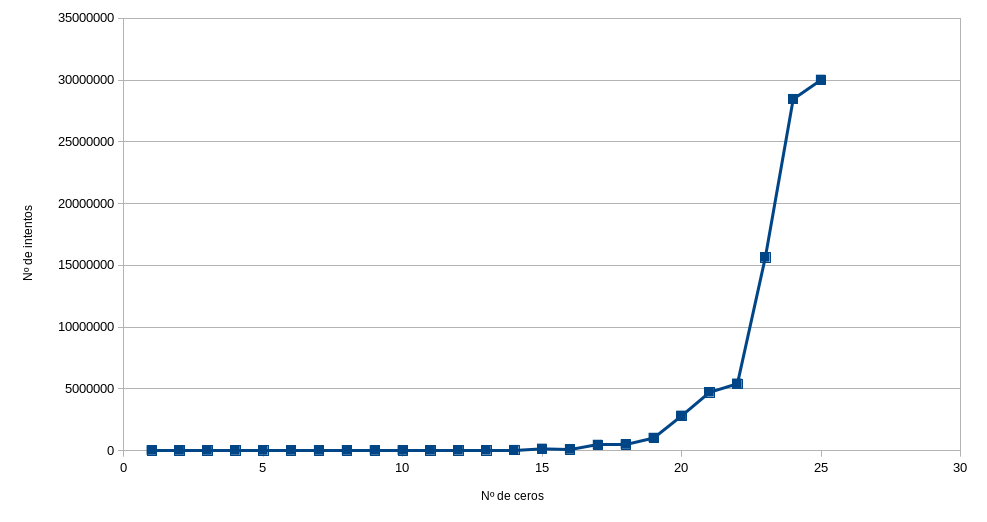
\includegraphics[width=1\textwidth]{./Imagenes/grafica_1.png}
\end{figure}

\noindent
Se puede observar como a partir de la búsqueda de cadenas con diecinueve ceros delante empieza a subir el número de intentos y a partir de veintitres se dispara.

% ----------------------------------------------------------------
\chapter{Ejercicio 3}

\section{Enunciado}
\noindent
Repetid la función anterior con el siguiente cambio: Se toma un primer valor aleatorio x y se va incrementadno de 1 en 1 hasta obtener el hash requerido.

\section{Respuesta}
\noindent

% ----------------------------------------------------------------
\chapter{Ejercicio 4}

\section{Enunciado}
\noindent
Calculad una nueva tabla/gráfica similar a la obtenida en el punto 2 pero con la función construida en 3.

\section{Respuesta}
\noindent

% ----------------------------------------------------------------
\end{document}
